\begin{frame}[t,fragile]{擬似乱数生成器における相関}
  \begin{itemize}
    %\setlength{\itemsep}{1em}
  \item 合同乗算法で多次元超立方体中に「ランダムに」点を打つと、それらの点は全て比較的小数の等間隔に並んだ超平面の上にのってしまう (多次元疎結晶構造)
  \resizebox{!}{.35\textheight}{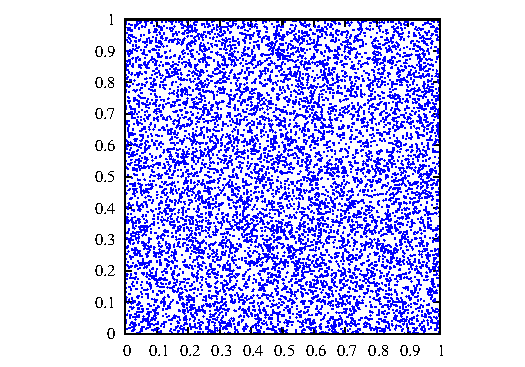
\includegraphics{image/lcg-2d.pdf}}
  \resizebox{!}{.35\textheight}{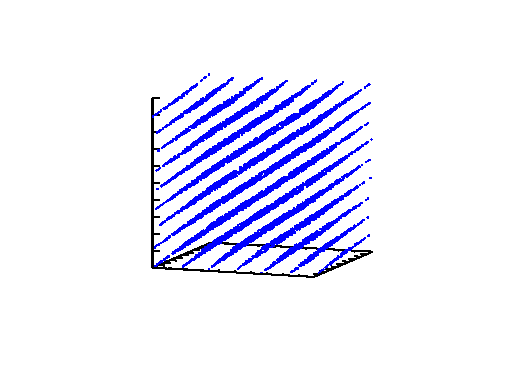
\includegraphics{image/lcg-3d.pdf}}
  \item 計算式に従って生成するため、必ず何らかの相関は残る
  \item できる限り相関が少なく周期の長い、理想的な乱数の開発が続けられている
    \begin{itemize}
    \item 現時点で、標準的な乱数発生器:メルセンヌ・ツイスター
    \item 周期 $2^{19937}-1$、高速、日本製! (例: \href{https://github.com/todo-group/computer-experiments/blob/master/exercise/monte_carlo/random.c}{random.c})
    \end{itemize}
  \end{itemize}
\end{frame}
